\section{Android: Entwicklung für die OpenSource-Welt}
\label{android}

\subsection{Was ist Android?}
Das Betriebssystem \textit{Android} basiert auf dem Linux-Kernel und ist seit 2012 das am meisten
verwendete Betriebssystem für Smartphones mit einem Marktanteil von etwa 70\%.

\begin{figure}[H]
  \begin{center}
    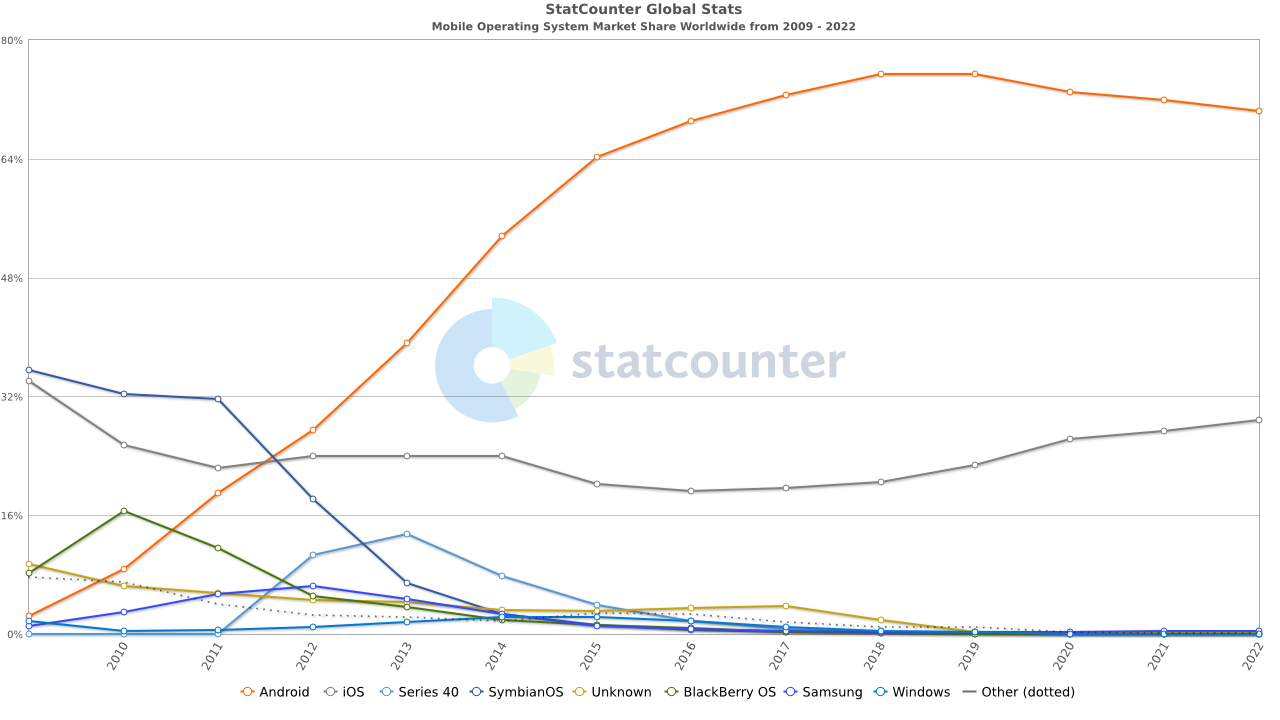
\includegraphics[width=0.6\textwidth]{Theorie/Android/mobileOsMarketShare.png}
    \caption{Mobilgeräte Betriebssysteme Marktanteile \cite{mobileOsMarketShare}}
  \end{center}
\end{figure}

\textit{Android} selbst ist freie Software \cite{androidOpenSourceProject}, welche dadurch definiert
ist, dass jeder Anwender die Software für jeden Zweck verwenden, alle Teile des Quellcodes
ändern und das Ergebnis kopieren und verteilen darf. Jedoch werden die meisten Android-Mobilgeräte
mit vorinstallierter, nicht-freier Software von den Geräte-Herstellern ausgestattet, was die
eigentliche Installation auf dem Gerät proprietär macht.

\subsection{Geschichte}
Im Jahre 2008 veröffentlichte \textit{Google LLC} die erste Version des Betriebssystems, welches
zuvor von Andrew Rubin für die Steuerung von Digitalkameras entwickelt wurde. Es sollte in den
nachfolgenden Jahren von der \textit{Open Handset Alliance}, einem Unternehmenszusammenschluss
aus Firmen im IT-Sektor, weiterentwickelt werden und offene Standards für Mobilgeräte festlegen.

\subsection{Verwendung}
\textit{Google} stellt selbst eine Reihe von Mobilgeräten her, darunter bis 2015 das Nexus und
heutzutage das Google Pixel, mit dem Google Pixel 6 Pro als Flaggschiff von 2021. Die Smartphones
sind mit einer Basis-Version von Android ausgestattet, wohingegen die Tablets und Notebooks Chrome
OS verwenden.

Viele Geräte-Hersteller entwickeln und pflegen eine eigene Abwandlung des Android Open Source
Projekts, sogenannte Aufsätze. Dabei werden meistens Elemente der Benutzeroberfläche stark, jedoch
der grundsätzliche Aufbau gar nicht bis minimal verändert. Bekannte Android-Aufsätze sind:

\begin{itemize}
  \item One UI von Samsung (Südkorea)
  \item MIUI von Xiaomi (China)
  \item EMUI von Huawei (China)
  \item OxygenOS von OnePlus (China)
\end{itemize}

\subsection{App-Entwicklung}
Der offizielle und empfohlene Weg, um eine native Android-Anwendung zu erstellen, ist das
Android Software Development Kit (SDK), zu deutsch Android Softwareentwicklungspaket. 
